\documentclass[%
onecolumn,
11pt,
tightenlines,
%reprint,
notitlepage,
superscriptaddress,
%groupedaddress,
%unsortedaddress,
%runinaddress,
%frontmatterverbose, 
%preprint,
%showpacs,preprintnumbers,
nofootinbib,
%nobibnotes,
%bibnotes,
amsmath,amssymb,
aps,
pra,
%prb,
%rmp,
%prstab,
%prstper,
%floatfix,
]{revtex4-1}


\def\andname{\hspace*{-0.5em},}

\setcitestyle{authoryear,round}
%% Language and font encodings
\usepackage[english]{babel}
\usepackage[utf8x]{inputenc}
\usepackage{textgreek}
\usepackage[T1]{fontenc}
\usepackage{physics}
\usepackage{graphicx}
\usepackage[colorlinks]{hyperref}
\usepackage{natbib}
\hypersetup{
    allcolors = blue,
}
\bibliographystyle{apj}
\usepackage{color}
\usepackage{array}
\usepackage{float}
\usepackage{gensymb}
\usepackage{todonotes}
\usepackage{ads}

\def\bibsection{\section*{REFERENCES}}

\begin{document}
\title{Investigating the Potential for a Milky Way Radio Halo}
\author{Nitika Yadlapalli}
\author{Vikram Ravi}
	\affiliation{Department of Astronomy, California Institute of Technology}


\begin{abstract}
\vspace{2mm}
This work seeks to investigate the source of the excess radio background emission reported in the ARCADE 2 results. While ARCADE 2 and similar experiments in the past used a plane-parallel slab model to explain the galatic forground, we use a disk and halo model to test for the existence of a Galactic radio halo in addition to a background. Such a halo might form via cosmic rays from the plane of the Galaxy diffusing out along magnetic field lines, and would leave a specific geometric signature in the sky brightness. Fits to all-sky maps in both image space and spherical harmonics space were attempted using Python packages \texttt{emcee} and \texttt{healpy}, though the presence of nearby Galactic features as well as poorly understood systematics in the maps makes those results inconclusive. We also fit to data from another experiment, TRIS, which measures sky brightness along a single declination strip. Both of these techniques show preliminary evidence for the existence of a halo, though further study is required to conclusively state the physical meaning of these results.

\end{abstract}

\maketitle

\section{Introduction}
All-sky maps exist for a broad range of radio frequencies and are typically expressed in brightness temperature, as shown in equation~\ref{Tsky}, where $\nu$, $l$, and $b$ are frequency, Galactic longitude, and Galactic lattitude respectively. Brightness temperature is defined as the temperature of a blackbody that would produce a given specific intensity at a given frequency. In radio frequencies, it is expressed as the Rayleigh-Jeans tail of the blackbody function (equation~\ref{RJ}).

\begin{equation}
T_{sky}\left(\nu,l,b\right) = T_{gal}\left(\nu,l,b\right) + T_{EG}\left(\nu\right) + T_{CMB}
\label{Tsky}
\end{equation}

\begin{equation}
T_{b} = \frac{I_{\nu}c^{2}}{2k\nu^{2}}
\label{RJ}
\end{equation}

Thus, experiments interested in measurements pertaining to the CMB must take care to accurately subtract off contributions from extragalactic sources and the Galaxy. A balloon experiment from 2006, the Absolute Radiometer for Cosmology, Astrophysics and Diffuse Emission (ARCADE 2), sought to measure deviations from the CMB's blackbody spectrum at frequencies lower than other CMB missions, like \emph{COBE}/FIRAS \citep{Fixsen2011}. ARCADE 2 observed in five frequency bands (3, 8, 10, 30, and 90 GHz) and made use of an external blackbody calibrator in order to characterize instrumental effects. Galactic emission was modelled with a plane-parallel slab model, where brightness temperature, $T_{b}$, is a linear function of $csc(b)$ where $b$ is Galactic latitude \citep{Kogut2011}. After applying this model for the Galaxy, and subtracting off brightness temperature contributions from the CMB and extragalactic sources, the ARCADE 2 team finds approximately 0.5 K excess temperature of unknown origin at 1 GHz \citep{Seiffert2011}. Several theories have been proposed for this excess, many of which are summarized in \cite{Singal2018}, but the one of interest in this report is the possibility of a Galactic synchrotron halo. 

The theory for a Galactic radio halo dates back as far as the mid-1900s. \cite{Ginzburg1961} suggest the existence of a Galactic halo composed of cosmic rays with a radius of around 10 kpc. They believe cosmic rays originate in the disk and travel along magnetic field lines into the halo. As the halo is predicted to be spherical/ellipsoidal, this implies disordered magnetic fields in the disk, from where the particles originate, as well as the halo. As long as the particles diffuse out of the disk faster than their synchrotron lifetimes, a synchrotron halo would be observed. 
Certain doubts about this theory were also raised. It was suggested that observations of the halo were a result of poor instrument resolution and also that there existed an insufficient number of electron-accelerating regions (such as type II supernovae) to explain the observed radio emission \citep{Mills1959}. Over time, interest in this question faded until the ARCADE 2 results, which brought renewed enthusiasm to the field.

One method of testing the existence of a Galactic halo would be to attempt to fit a disk/halo geometry to current all-sky maps. Such an analysis of modelling the sky using two spheroids, one for the disk and one for the halo, was done by \cite{Subrahmanyan2013}. A variation on that analysis is performed in this study as well.

Similar to ARCADE 2, another absolutely calibrated experiment called TRIS observed a circle on the sky at a constant declination of 42$\degree$ and $\nu$ = 0.6, 0.82, and 2.5 GHz \citep{Zannoni2008}. Rather than trying to create a model of the Galaxy, the TRIS team came up with a method of subtracting off the Galactic component from the uniform component just using their data. First, they generate a TT plot for two different frequencies, a method introduced by \cite{Turtle1962}. A TT plot graphs brightness temperatures at the same coordinates but at two different frequencies. The TRIS team plotted $T_b$(0.82 GHz) vs. $T_b$(0.6 GHz). The TT plot can be used to determine a spectral index of Galactic emission. As the background formed by the CMB and unresolved extragalactic sources is homogeneous, it theoretically contributes only one point to the TT plot. Any variations in temperature will be due to structure in the Galaxy, which then form most of the distinct points in the TT plot. Often, a few different trends can be seen on the plot, indicating variation in spectral index as a function of position. This can be used to separate the observed brightness temperature into contributions from the Galaxy and contributions from the background. A derivation of this is given in \cite{Gervasi2008} and \cite{Tartari2008}. The TRIS team reports no excess background temperature.

A radio halo in our own Galaxy could give us insight into the formation mechanisms of similar halos observed in other galaxies.The Continuum Halos in Nearby Galaxies, an EVLA Survey (CHANG-ES), for example aims to study extragalactic radio halos. They find that many of the edge-on spiral galaxies they observed exhibited synchrotron halos \citep{Wiegert2015}. Should evidence of such a halo be found for the Milky Way as well, we would be in a unique place to study the origins of radio halos.

This report is organized as follows. First, we discuss our models of the Galactic foreground as well as our calculations for brightness temperature of extragalactic sources. We then discuss fitting model parameters to all-sky maps and the limitations of those analyses. We then discuss similar analyses carried out for data taken by TRIS. A brief discussion of results is given for each section.


\section{Methods}
\subsection{Disk and Halo Models}
In order to fit disk and halo models to currently available observations, we first needed to come up with models calculated from the perspective of the earth. By assuming an isotropic emissivity and by calculating the line of sight distance through the disk and halo, we can calculate the predicted brightness temperature from the model in all directions via equations \ref{I_v} - where $I_{\nu}$ is the specific intensity, $j_{\nu}$ is the emission coefficient of the disk/halo, and $D$ is the line of sight distance through the disk/halo - and \ref{RJ}, the Rayleigh-Jeans limit of the Planck function.
\begin{equation}
I_{\nu} = j_{\nu}D
\label{I_v}
\end{equation}

We initially assumed a cylindrical model for the Galactic disk. The line of sight distance would be dependent on the radius of the cylinder, $R_{disk}$, the height, $h_{disk}$, distance from the Galactic center, $d$, and Galactic longitude and latitude, $l$ and $b$. In some instances, we found a spheroidal model for the disk to be preferabe to the cylindrical one. For the spheroidal models, we assume that $R_{disk}$ represents the semi-major axis while $h_{disk}$ represents the semi-minor axis. For comparison, an example for each model, given the same geometric values and emissivity, is shown in Fig~\ref{disk_models}. For the halo, we assume a spherical geometry. An example of this model is shown in Figure~\ref{halo_model}.


\begin{figure}[h]
\begin{center}
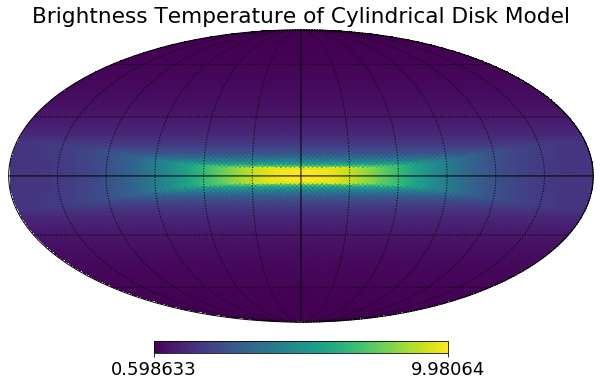
\includegraphics[width=0.49\textwidth]{example_disk.jpg}
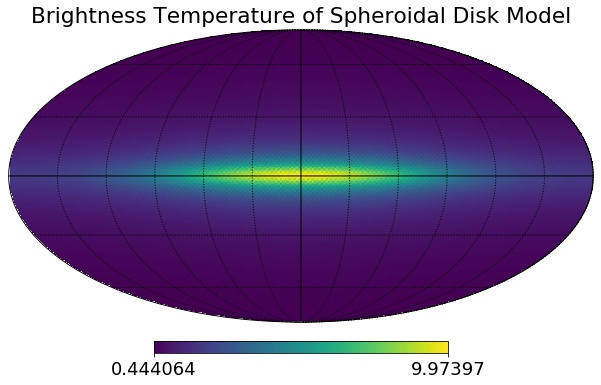
\includegraphics[width=0.49\textwidth]{example_sph.jpg}
\caption{Two examples of models for a Galactic disk. On the left is a cylindrical model while on the right is a spheroidal model}
\label{disk_models}
\end{center}
\end{figure}

\begin{figure}[h]
\begin{center}
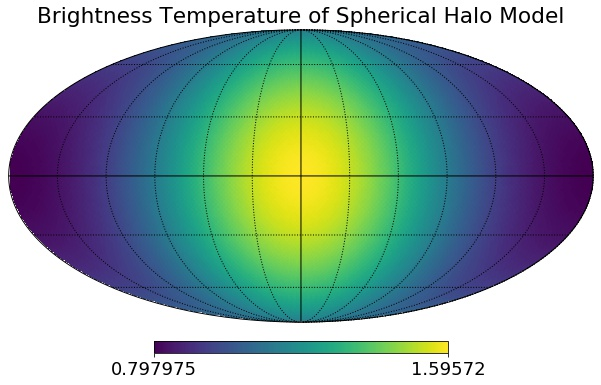
\includegraphics[width=0.49\textwidth]{example_halo.jpg}
\caption{An example of a model for a Galactic halo.}
\label{halo_model}
\end{center}
\end{figure}



\subsection{Extragalactic Temperature Contribution}
In order to calculate the total brightness contributed by extragalactic sources, several models covering source counts for different brightness ranges were combined. Source counts in the range of 0.05 - 1000\ mJy can be modelled by the sixth order polynomial described by equation~\ref{Hopkins} \citep{Hopkins2003}. 

\begin{equation}
log\left(\frac{dN/dS}{S^{-2.5}}\right) = -0.008x^{6} + 0.057x^{5} - 0.121x^{4} - 0.049x^{3} + 0.376x^{2} + 0.508x + 0.859 \\
\label{Hopkins}
\end{equation}

\begin{equation*}
x = log\left(\frac{S}{mJy}\right)
\end{equation*}

In the range of $0.011-44$ mJy, \cite{Smolcic2017} reports specific values for $\frac{dN/dS}{S^{-2.5}}$ at various sky brightnesses. Finally, in the range of $ S < 10\ \mu$Jy, \cite{Condon2012} predicts that the source counts at 3.02 GHz are described by equation~\ref{Condoneq}.

\begin{equation}
\frac{dN}{dS} = 9000S^{-1.7}\ Jy^{-1}\ sr^{-1}
\label{Condoneq} 
\end{equation}

As these equations describe source counts at various frequencies, we need to use equation~\ref{spectralindex} to transform $S$ into the frequency of our choice, where the spectral index is $ \alpha = -0.7$ \citep{Condon2012}.

\begin{equation}
S_{f} = S_{i} \left(\frac{\nu_{f}}{\nu_{i}}\right)^{\alpha}
\label{spectralindex}
\end{equation}

Once all of the brightnesses are at a consistent frequency, equation~\ref{StoT} describes how to calculate the final integrated brightness temperature. A plot representing the differential temperature is shown in Figure~\ref{Tb}.

\begin{equation}
T_{b} = \int \left(\frac{dT}{dS}\right) dS \ = \int \left(S\frac{dN}{dS}\right) \frac{c^{2}}{2\nu^{2}k} dS
\label{StoT}
\end{equation}

\begin{figure}[h]
\begin{center}
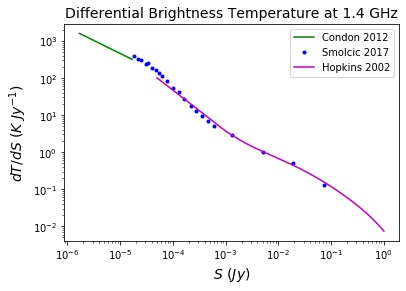
\includegraphics[width=0.5\textwidth]{T_b.jpg}
\caption{Differential brightness temperature plotted as a function of source brightness at 1.4 GHz}
\label{Tb}
\end{center}
\end{figure}


\section{Results and Discussion}

\subsection{Fitting to Images}
Our first attempt to fit a disk+halo Galaxy model to an all-sky radio image was to a 1.4 GHz map \citep{Reich1986} downloaded from NASA's LAMBDA database. This map was genereated using data from two telescopes in order to get full coverage of both the northern and southern sky. Data for the northern sky was taken with the Stockert 25 m telescope, while data for the southern sky was taken with a 30 m telescope in Villa Elisa. In order to assess the fit, we need to analyze the residuals, calculated in equation~\ref{T_res}, where the $T_{bkg}$ is a free parameter meant to represent any excess uniform emission. 

\begin{equation}
T_{residual}(l,b) = T_{sky}(l,b) - \left(T_{disk}(l,b) + T_{halo}(l,b)\right) - T_{extragalactic} - T_{CMB} - T_{bkg}
\label{T_res}
\end{equation}

\begin{figure}[b]
\begin{center}
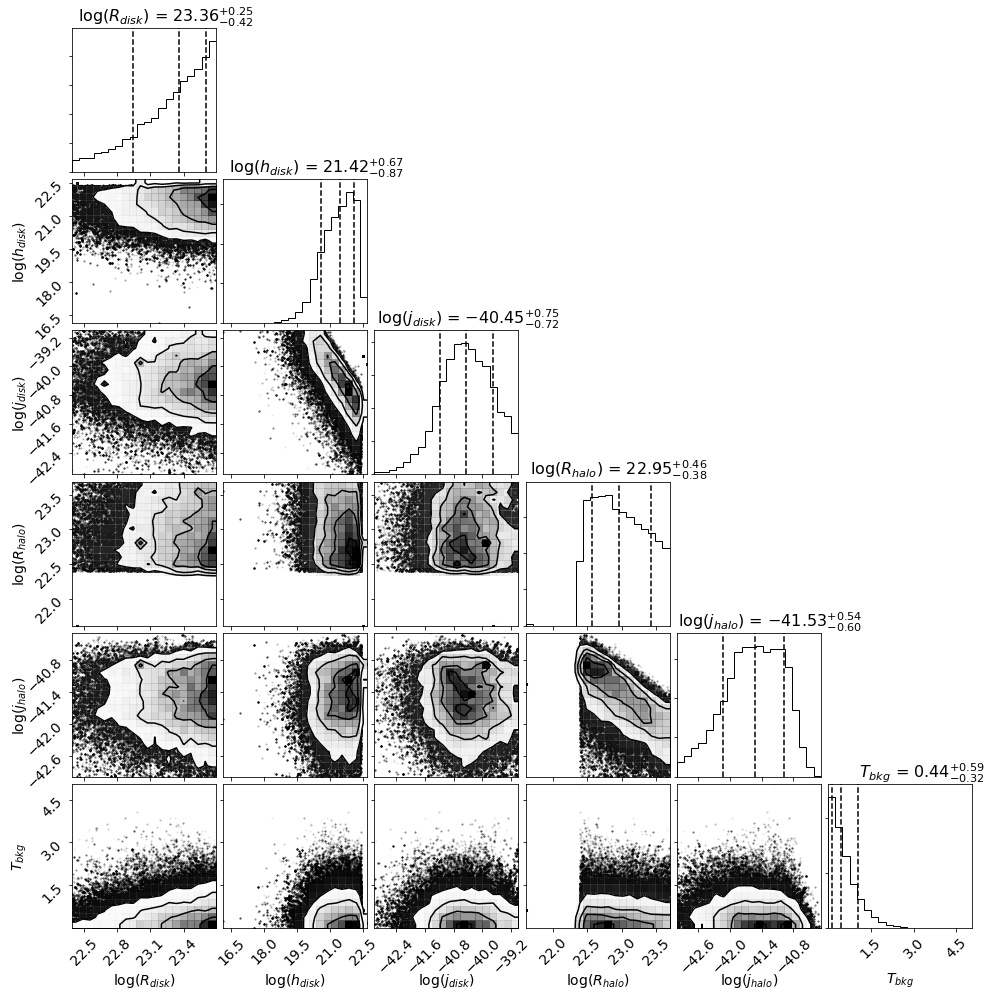
\includegraphics[width=0.8\textwidth]{corner_disk+halo+bkg.jpg}
\caption{Corner plot showing the results from the MCMC analysis of the 1.4 GHz all sky map assuming a disk, halo, and uniform background model for the Galaxy.}
\label{corner_disk+halo+bkg}
\end{center}
\end{figure}


\begin{figure}[b]
\begin{center}
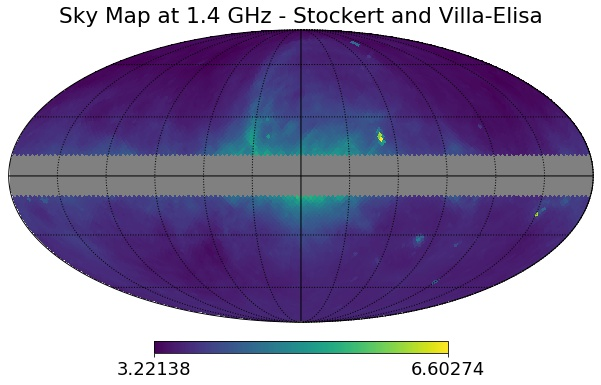
\includegraphics[width=0.47\textwidth]{1420_map.jpg}\\
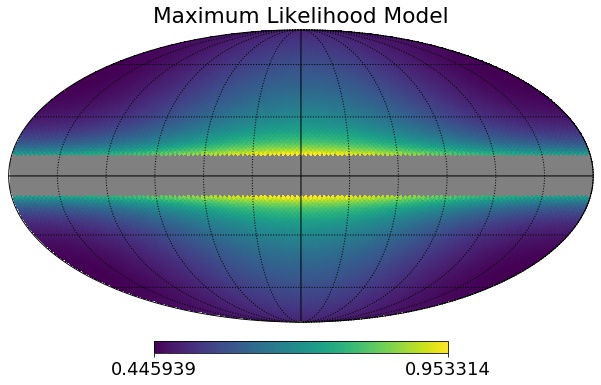
\includegraphics[width=0.47\textwidth]{1420_model.jpg}\\
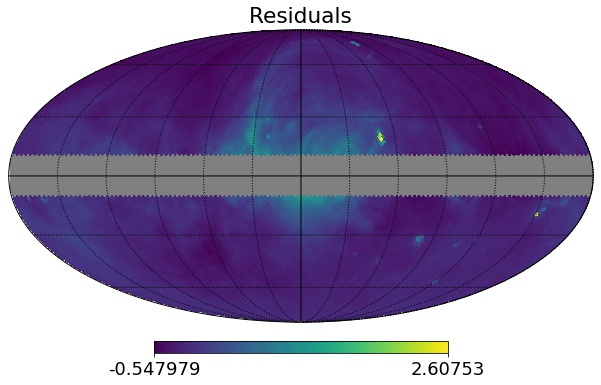
\includegraphics[width=0.47\textwidth]{1420_residuals.jpg}
\caption{Maps of the 1.4 GHz sky, the best fit model as calculated by MCMC, and the residuals}
\label{1420maps}
\end{center}
\end{figure}


For an ideal model, the sky temperature minus the model temperature should just leave Gaussian noise. In reality, it is impossible for our rudimentary models to subtract  features such as loops and spurs, so we will be left with more positive residuals than negative. The residuals should follow a right-tailed distribution, where the negative residuals resemble half a Gaussian and the positive residuals include residual emission caused by specific features, such as the loops and spurs. So, to assess the fit, we measure the Gaussianity of the negative residuals with a Kolmogorov-Smirnov test (KS test). This statistical test measures the maximum distance between the cummulative distribution function of the residuals and an empirical distribution function (EDF). The larger this maximum distance, the lower the p-value of the test. In order to find the set of parameters that best represent the data, we perform an MCMC analysis, using Python package \texttt{emcee}  \citep{emcee}, with the negative of the p-value of the KS test being the statistic we wish to minimize. This analysis involved six free parameters: $R_{disk}$, $h_{disk}$, $j_{disk}$, $R_{halo}$, $j_{halo}$, and $T_{bkg}$. As emission towards the Galactic center is dominated by foreground structure, the central 20$\degree$ of latitude were not included in the analysis. However, this led to a poor constraint on the best fit for $R_{disk}$, the best fit for which was calculated to be around 9.2$d$ (where $d$ is the distance to the Galactic center). This is because the peak brightness of the data, which would provide an upper limit on $R_{disk}$, was masked. The most likely values for the thickness of the disk and the radius of the halo were 0.1$d$ and 3.6$d$, respectively. The thickness of the disk in kiloparsecs is 0.85 kpc, which is significantly greater than the 0.3 kpc expected for the stellar disk. Additionally, the best fit for the emission coefficients predict the disk to be order of magnitude more emissive than the halo. The results of the MCMC analysis also show the maximum likelihood of $T_{bkg}$ is 0 K, indicating that there may be no excess emission left unexplained after including a halo in the model of the Galaxy. The resulting corner plot from the analysis is shown in Figure~\ref{corner_disk+halo+bkg} while maps of the original sky brightness, the model, and residuals are shown in Figure~\ref{1420maps}. 

In a separate MCMC analysis of a disk and background only model (no halo), the Markov chain for background temperature showed a maximum likelihood of $0.65^{+0.67}_{-0.41}$ K. This is fairly close to the 0.5 K excess reported by the ARCADE 2 team, however the prediction has a large error. The absence of this background in the analysis including contributions from the halo may indicate some merit in the halo model, but further investigation is needed to confirm.

In addition to an attempt to fit the models in image space, a fit in spherical harmonics space was also attempted. Using Python package \texttt{healpy}'s spherical harmonics transforms, coefficients for the sky map and the models are computed. Then, the error in the coefficients is minimized, with the coefficients weighted according to the "noise" in that coefficient as dictated by the power spectrum, to find the best fit using MCMC. In both of these cases, however, systematic effects present in the 1.4 GHz map make assessing the validity of the results difficult. Firstly, this map is constructed from observations taken from two different telescopes. These telescopes have different beam sizes and different calibrations, making the data between the northern and southern hemispheres potentially inconsistent. In order to perform an independent check of the results found here, a similar analysis was done on the TRIS 0.6 GHz dataset. 

\subsection{Fitting to TRIS Data}

% show original vs galaxy subtraction plot
% describe MCMC analysis (integral of abs value residuals)

The TRIS team observed the sky at a constant declination ($\delta$ = 42$\degree$) and thus, were able to create plots of brightness temperature as a function of RA. They then used the methods outlined in \cite{Gervasi2008} to calculate the temperature of the Galactic foreground at every RA. A plot showing the temperatures of the sky and Galaxy together at 0.6 GHz is shown in Figure~\ref{TRIS_Tgal}. We are now interested in fitting a disk and halo model to this data. An advantage of the TRIS dataset is that it avoids areas with large, nearby features. As there are too few data points in the TRIS dataset to use the KS test as our test statistic, we instead use an integral of the absolute value of the residuals, as quantified by equation~\ref{TRIS_res}, as the statistic we wish to minimize.
Two separate MCMC anaylses were performed, one with just a disk and one with a disk and a halo. It should be noted that in this analysis, a spheroidal disk was preferred to a cylindrical disk. A spheroidal disk has a brightness temperature as a function of RA that is smooth everywhere, whereas a cylindrical disk exhibits a cusp.


\begin{equation}
T_{res} = T_{gal} - \left(T_{disk} + T_{halo}\right)
\label{TRIS_res}
\end{equation}


The highest likelihood model compared to the true sky temperature for both cases are shown in Figure~\ref{TRIS_MCMC}. The peaks are reasonably well modelled in both cases, however the region between 150$\degree$~<~RA~<~250$\degree$ is only modelled accurately in the case of a disk+halo. The disk alone model fails to model the postitive slope in brightness temperature. The corner plot visualing the values of the parameters for the disk+halo model is shown in Figure~\ref{corner_TRIS_sph+halo}. The highest likelihood values for $R_{disk}$ and $R_{halo}$ are about 17.4 kpc (2.2$d$) and 18.2 kpc (2.3$d$) respectively. The radius of the disk is much lower than that predicted from the KS test, due to the fact that the data was more constraining. The radius of the halo is also lower in this analysis. The most likely value for $h_{disk}$, however, is around 6.84 kpc (0.86$d$), indicating a very thick disk compared to the disk predicted from the KS test. The thickness of the disk may be overpredicted, however, to compensate for extra brightness contributed by the Cygnus-X star forming region, located in the Galactic plane and the cause of the peak around RA=300$\degree$. Future analyses may involve masking this region. One consistent result between the two analyses is that the emission coefficient of the disk is about an order of magnitude larger than that of the halo. Further work is necessary to interpret these results.

\begin{figure}[H]
\begin{center}
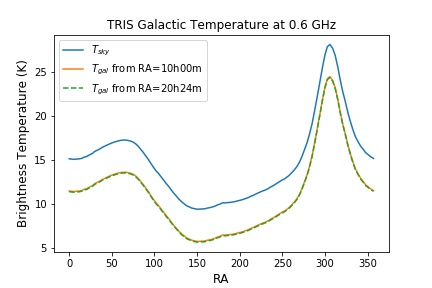
\includegraphics[width=0.5\textwidth]{TRIS_Tgal.jpg}
\caption{Temperature of sky and Galactic foreground as a function of RA, as measured by TRIS at 0.6 GHz. Galactic temperature is calculated using two separate reference locations.}
\label{TRIS_Tgal}
\end{center}
\end{figure}

\begin{figure}[H]
\begin{center}
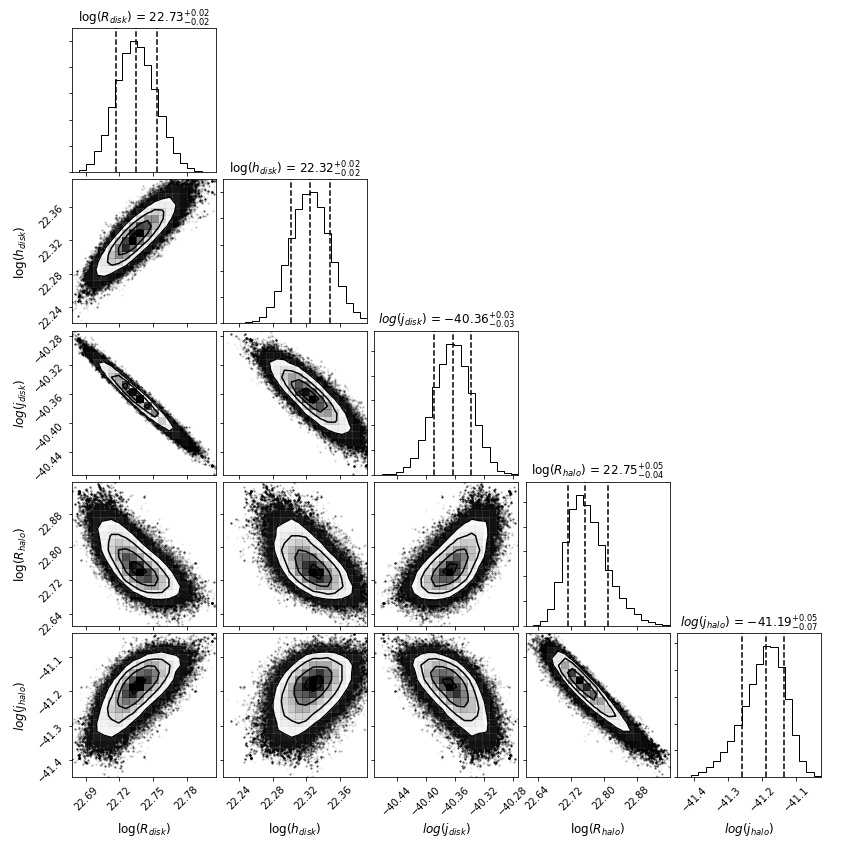
\includegraphics[width=0.7\textwidth]{corner_TRIS_sph+halo.jpg}
\caption{Corner plot showing the results from the MCMC analysis of the 0.6 GHz TRIS data, with the uniform background subtracted off, assuming a disk and halo model for the Galaxy.}
\label{corner_TRIS_sph+halo}
\end{center}
\end{figure}

\begin{figure}[t]
\begin{center}
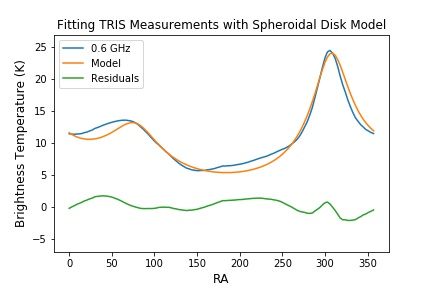
\includegraphics[width=0.495\textwidth]{residuals_TRIS_sph.jpg}
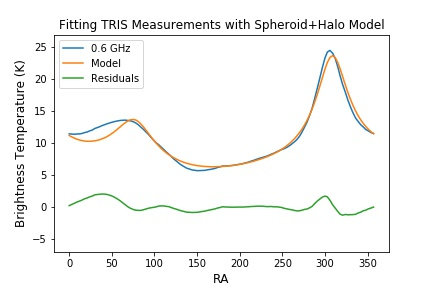
\includegraphics[width=0.495\textwidth]{residuals_TRIS_sph+halo.jpg}
\caption{Residuals of the best fits, as calculated by the MCMC analysis, for a disk only model (left) and disk+halo model (right).}
\label{TRIS_MCMC}
\end{center}
\end{figure}

\section{Conclusion}
This report presents results of using a Galactic radio halo in attempts to explain the excess radio background reported by ARCADE 2. Fits to an all-sky 1.4 GHz map in image space showed the existence of a uniform background with a disk only model, which was not present in a disk+halo model. However, these results may be biased by the presence of bright features, such as the North Galactic spur, as the MCMC walkers may be attempting to model these features rather than overall Galaxy structure. To avoid this and other systematics affecting all-sky maps, a similar analysis was done with the TRIS dataset, as the TRIS observing path avoids emission from the North Galactic Spur. Comparing the disk only model with the disk+halo model and the TRIS sky brightness data shows that the emission profile is best fit with the presence of the halo. These results are still preliminary, however, and statistical tests of model selection are necessary before any confident conclusions about the presence of the radio halo can be made.

% while no absolute conclusion can be reached about the size of a galactic halo, compelling evidence (esp from the TRIS data) exists that a halo is necessary to explain the emission profile

%\begin{acknowledgments}
%\end{acknowledgments}

\bibliography{QualReportBib}

\end{document}